\subsection{Vergleich zum O(1)-Scheduler}\label{s:compO1}
In den letzten Jahren ist der Anteil an Nutzern, die Linux als Desktop-Version einsetzen stetig gestiegen. Daher war es auch an der Zeit den CPU-Scheduler hinsichtlich Interaktivität zu verbessern. Unter anderem diesen Ansatz verfolgte Ingo Molnár mit der Entwicklung des O(1)-Sche\-dulers. Laut \cite{papercomparison} haben Studien gezeigt, dass in Desktop-Umgebungen die Antwortzeit des Systems als wichtiger erachtet wird als der Durchsatz. Für den Betrieb von interaktiven Anwendungen wird demnach eine sehr niedrige Latenz benötigt. 

Folgender Abschnitt folgt den Erläuterung aus \cite{asilberschatz} und \cite{papercomparison}. Die Diagramme sind aus \cite{papercomparison}.

Der O(1)-Scheduler arbeitet mit je einer Warteschlange (\textit{run queue}) pro Prozessor, die aus je einem aktiven und abgelaufenem (\textit{expired}) Array besteht. Um den nächsten Prozess zu bestimmen, der ausgeführt wird, wählt der Prozessor den Prozess mit der höchsten Priorität aus dem aktiven Array. Wenn es Aufgaben mit gleicher Priorität gibt, wird per Round-Robin ausgewählt. Die Arrays sind zweidimensional mit 140 Prioritätsleveln angeordnet. So gibt es für Realzeitaufgaben Prioritäten von 0 (hohe Priorität) bis 99 (niedrige Priorität). Die konventionellen, time-shar\-ing Prozesse befinden sich im Interval von 100-139 und bilden gleichzeitig die \textit{nice}-Werte von -20 bis 19 ab. Wenn das aktive Array leer ist, d.h. keine weiteren Aufgaben mehr wählbar sind, werden die Zeiger der Arrays getauscht und das aktive wird zum abgelaufenen und umgekehrt. Die statischen Prioritäten werden um dynamische ergänzt, indem der O(1)-Scheduler mittels einem Timer die durschnittliche \textit{sleep}-Zeit eines Prozesses misst und somit die Priorität im Array anpasst. Bei einem Ablauf einer Zeitscheibe eines Prozesses, wird die dynamische Priorität erneut kalkuliert, sodass bei einem Wechsel der Arrayzeiger die Elemente im Array mit den angepassten Prioritäten eingeordnet sind. \\
Um die Interaktivität zu verbessern, versucht dieser Scheduler  interaktive Prozesse zu identifizieren und anschließend zu bevorzugen. Dies geschieht anhand eines heu\-ris\-tisch\-en Deltas. Ist dieses kleiner oder gleich einem definierten Bonus, werden interaktive Aufgaben im aktiven Array gehalten obwohl deren Zeitquantum schon abgelaufen ist.

In Artikel \cite{papercomparison} haben die Autoren die beiden Scheduler hinsichtlich Fairness und Interaktivitätslatenz verglichen. Die Testszenarien und  Resultate aus \cite{papercomparison} werden im folgenden Abschnitt vorgestellt.

Für den Fairness-Test wurde gemessen, wie genau der Scheduler die CPU-Bandbreite über mehrere Prozesse verteilt. Dazu wurde ein Benchmark-Programm genutzt, welches eine diskrete Integralrechnung der Zahl Pi durchführt. Der Benchmark besteht dabei aus einem Elternprozess und $N$ Kindprozessen, die die Berechnung durchführen. Nach Erzeugen von $N$ Kindprozessen durch den Elternprozess, registrieren sich diese bei einem Signal-Handler. Durch ein Signal des Elternprozesses wird mitgeteilt, dass alle Kinder erzeugt worden sind und diese anschließend gleichzeitig mit der diskreten Integralrechnung beginnen. Es wird die Zeit in Nanosekunden gemessen, die jedes Kind für die Integralrechnung benötigt. Dabei werden vier Tests mit 8,16,24 und 32 Kindern à 100 Wiederholungen durchge\-führt. Als Testumgebung diente dabei ein Intel-Prozessor mit 2.13 GHz, 2GByte Arbeitsspeicher, einem Linux 2.6.22 für O(1) und Linux 2.6.24.2 für CFS. Es wurde nur ein Prozessorkern aktiviert, damit nur eine Warteschlange genutzt wird.  
\begin{figure} [h]
	\centering
	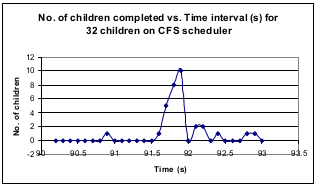
\includegraphics[width=0.45\textwidth]{pictures/fairness_32_cfs.png}
	\caption{Fairness-Messung für N=32 im CFS Scheduler.}
	\label{fig:fair_meas_cfs}
\end{figure}
\begin{figure} [h]
 	\centering
 	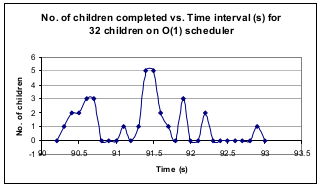
\includegraphics[width=0.45\textwidth]{pictures/fairness_32_O1.png}
 	\caption{Fairness-Messung für N=32 im O(1) Scheduler.}
 	\label{fig:fair_meas_o1}
\end{figure}

In den Abbildungen \ref{fig:fair_meas_cfs}\&\ref{fig:fair_meas_o1} sind die Ergebnisse bei $N=32$ zu sehen. Auf der X-Achse befinden sich die Zeitpunkte in Sekunden, an denen ein oder mehrere Kinder mit der Integralrechnung fertig waren. Korrespondierend dazu zeigt die Y-Achse, wieviele Kinder zum Zeitpunkt X fertig waren. Beispielsweise zeigt Abbildung \ref{fig:fair_meas_cfs}, dass nach ca. 92 Sekunden 10 Kinder mit der Berechnung fertig waren. Um auf die Gesamtanzahl von $N=32$ zu kommen, muss die angegebene Anzahl an fertigen Kindern pro Zeitpunkt über den gesamten Zeitrahmen summiert werden. \\
Zu erkennen ist, dass die Standardabweichung der gebrauchten Zeit pro Kind beim O(1)-Scheduler höher ist als die des CFS. Die weite Streuung der Daten im Diagramm \ref{fig:fair_meas_o1} zeigt, dass manche Kinder schneller fertig sind als andere. Die Kinder werden zu stark unterschiedlichen Zeitpunkten mit der Berechnung fertig.\\
Dahingegen sind die Daten im Diagramm zum CFS knapper und konzentrierter um den Spitzenwert angeordnet. CFS hat die CPU zu gleicheren Anteilen den Kindern zugeteilt, sodass diese ungefähr nach 92 Sekunden mit der Berechnung fertig waren. \\
Nach \cite{papercomparison} kann zusammenfassend gesagt werden, dass CFS die zur Verfügung stehende CPU-Zeit auf eine fairere Weise über jede Aufgabe verteilt. Die Autoren nennen als Grün\-de dafür, dass CFS die Zeitquanten sehr granular verteilt und diese in Nanosekunden berechnet werden.

Für die Messung der Interaktivitätslatenz wurde ebenfalls ein Benchmark genutzt, welches Interaktivitätsaufgaben und unterschiedliche Hintergrundaufgaben simuliert. Für die Interaktivitätslatenz wurde die Zeit gemessen, die zwischen dem Anfragen des Prozessors durch die interaktive Aufgabe und dem tatsächlichen Zeitpunkt des Erhalts der CPU liegt. Dies ist dann die Zeit, die der Scheduler benötigt, um die Ressource CPU für die interaktive Aufgabe zu allokieren. Im Test von \cite{papercomparison} wurden drei Tests durchgeführt: In jedem davon war die interaktive Aufgabe das X-Window System eines Linux-Betriebssystems und als Hintergrundaufgaben wurden drei verschiedene Belastungen simuliert. Im ersten Test war ein Abspielen einer Audiodatei mit 5\% CPU-Load, im zweiten das Abspielen eines Videos bei 60 frames/sec mit 40\% CPU-Load und abschließend eine volle Belastung bei 100\% simuliert. Auch hier wurde jeder Test 100 mal wiederholt und die Ergebnisse für die durschnittliche (arithmetisches Mittel) und die Maximallatenz in zwei Diagrammen (Abbildung \ref{fig:avg_latency}\&\ref{fig:max_latency}) dargestellt. 
\begin{figure} [h]
 	\centering
 	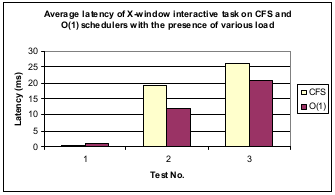
\includegraphics[width=0.45\textwidth]{pictures/avg_latency.png}
 	\caption{Durchschnittslatenz in CFS und O(1) Scheduler.}
 	\label{fig:avg_latency}
\end{figure}

\begin{figure} [h]
 	\centering
 	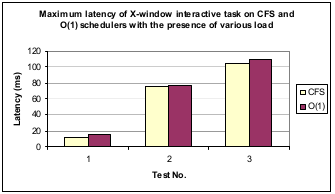
\includegraphics[width=0.45\textwidth]{pictures/max_latency.png}
 	\caption{Maximallatenz in CFS und O(1) Scheduler.}
 	\label{fig:max_latency}
\end{figure}
Als Resultat ist zu erkennen, dass CFS bei wenig Belastung eine niedrigere Durchschnittslatenz hat und bei mittlerer und höherer Belastung O(1) die niedrigeren Werte zeigt. Bei den Maximalwerten besitzt der CFS in allen drei Fällen niedrigere Werte als O(1). Jedoch liegen die hier gemessenen Werte immer noch weit unter der menschlichen Wahrnehmung (der Stimulus zum Hirn braucht schon 20-40ms), sodass ein Benutzer den Unterschied nicht bemerken würde. Es wurde gezeigt, dass obwohl der CFS keine Bervorzugung von interaktiven Aufgaben mehr vornimmt, die Interaktivitätslatenz vergleichbar zum O(1)-Scheduler ist. 

Insgesamt erklären die Autoren die bessere Effizienz des CFS dadurch, da dieser fairer zu allen Aufgaben im System ist und kein komplexen Algorithmus und keine Heuristiken benötigt, um interaktive Aufgaben zu identifizieren und diese zu bevorzugen.